%sample location map
\begin{figure}
\centering
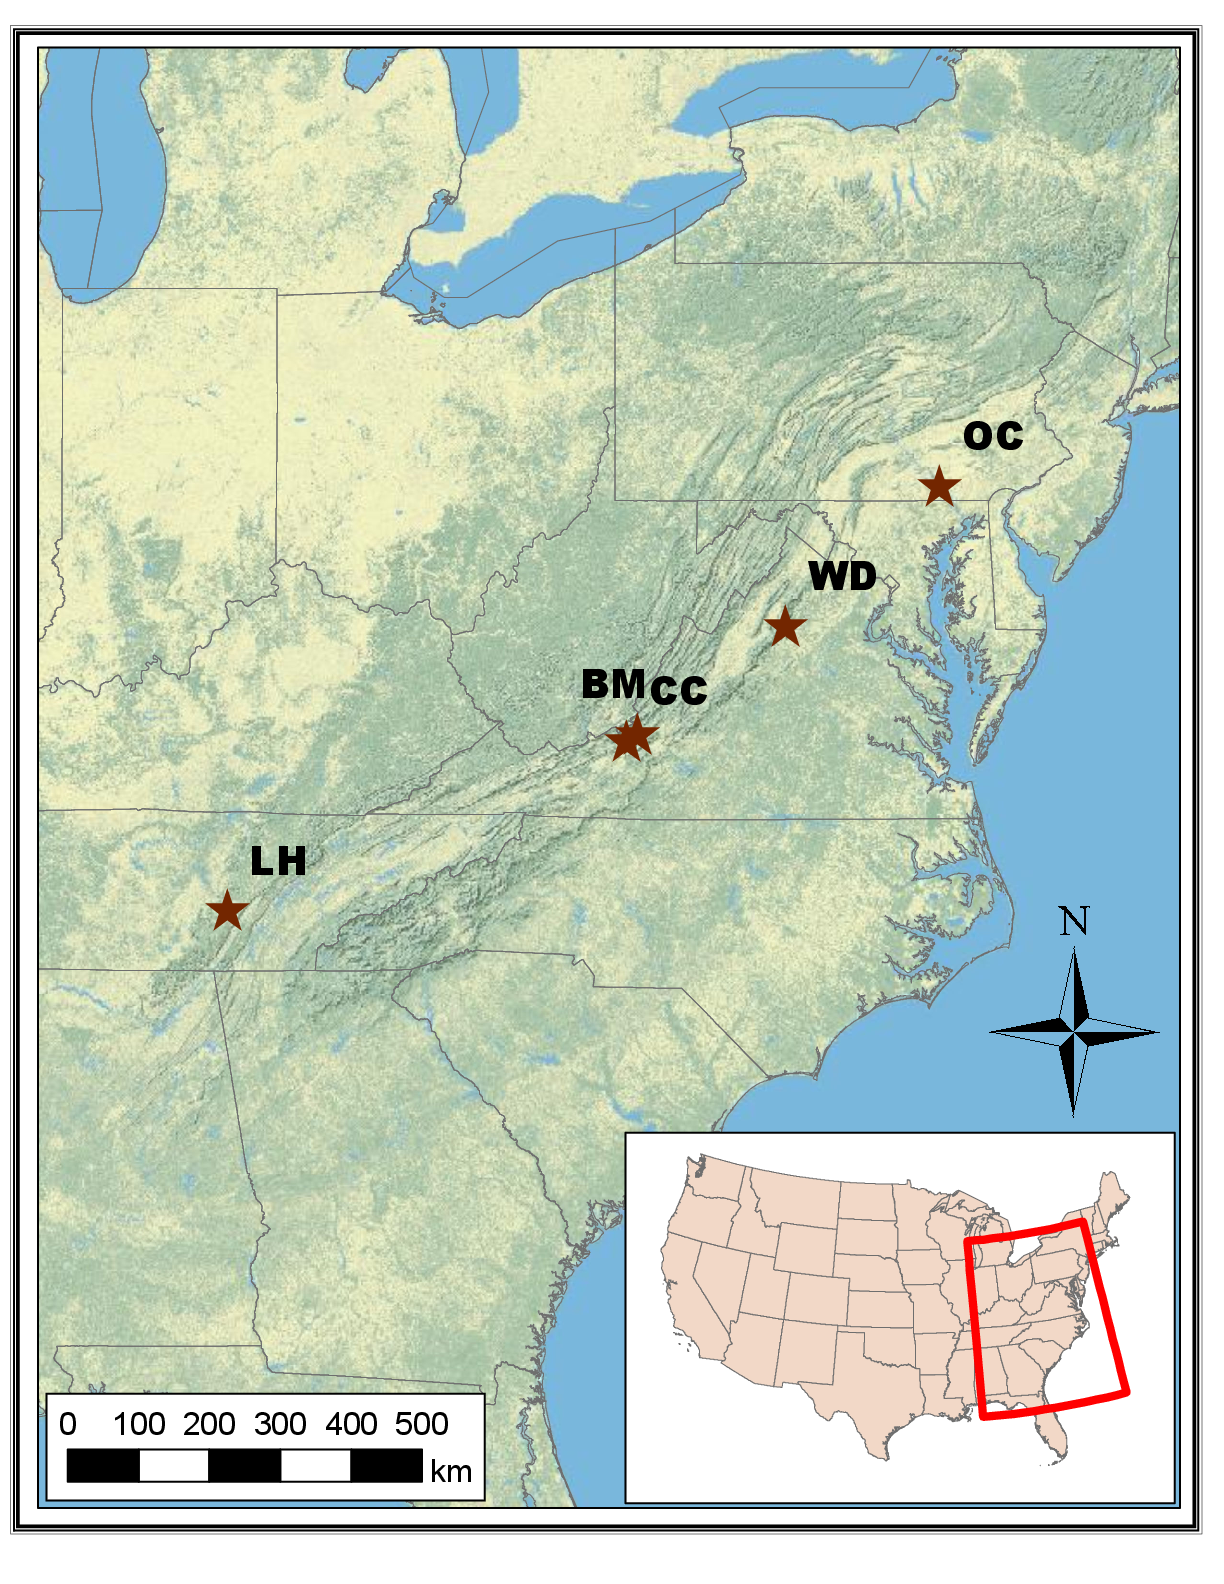
\includegraphics[width=5in]{figures/NewClimateNADEF.png}
\caption{Regional chronology sample locations.}
\label{fig:map}
\end{figure}

%chron time series plots
\begin{figure}
\centering
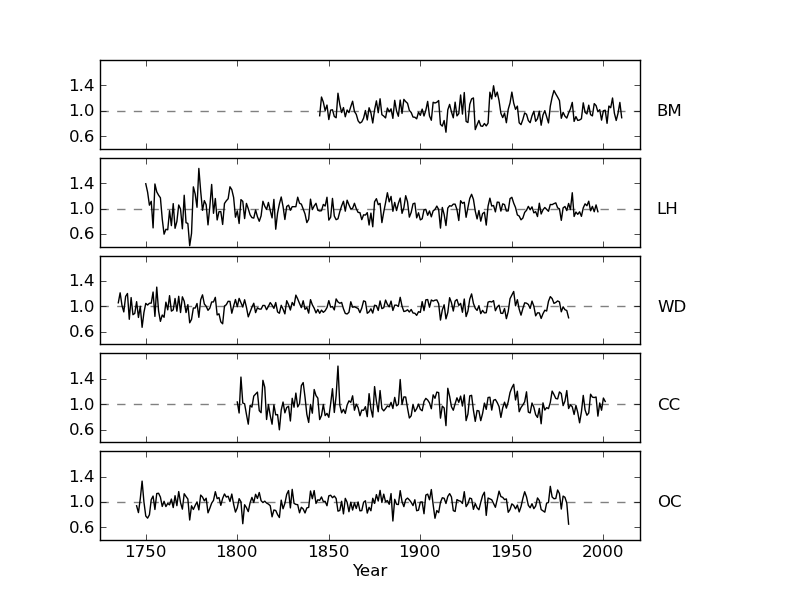
\includegraphics[width=5in]{figures/stacked_chrons.png}
\caption{Plots of the five chronologies used in the principal component analysis. The top panel shows the chronology built from the sample data at Brush Mountain (BM), while the others are the regional chronologies from Lynn Hollow (LH), Watchdog Mountain (WD), Craig Creek (CC), and Otter Creek (OC).}
\label{fig:stackedChrons}
\end{figure}

%climate correlation plot
\begin{figure}
\centering
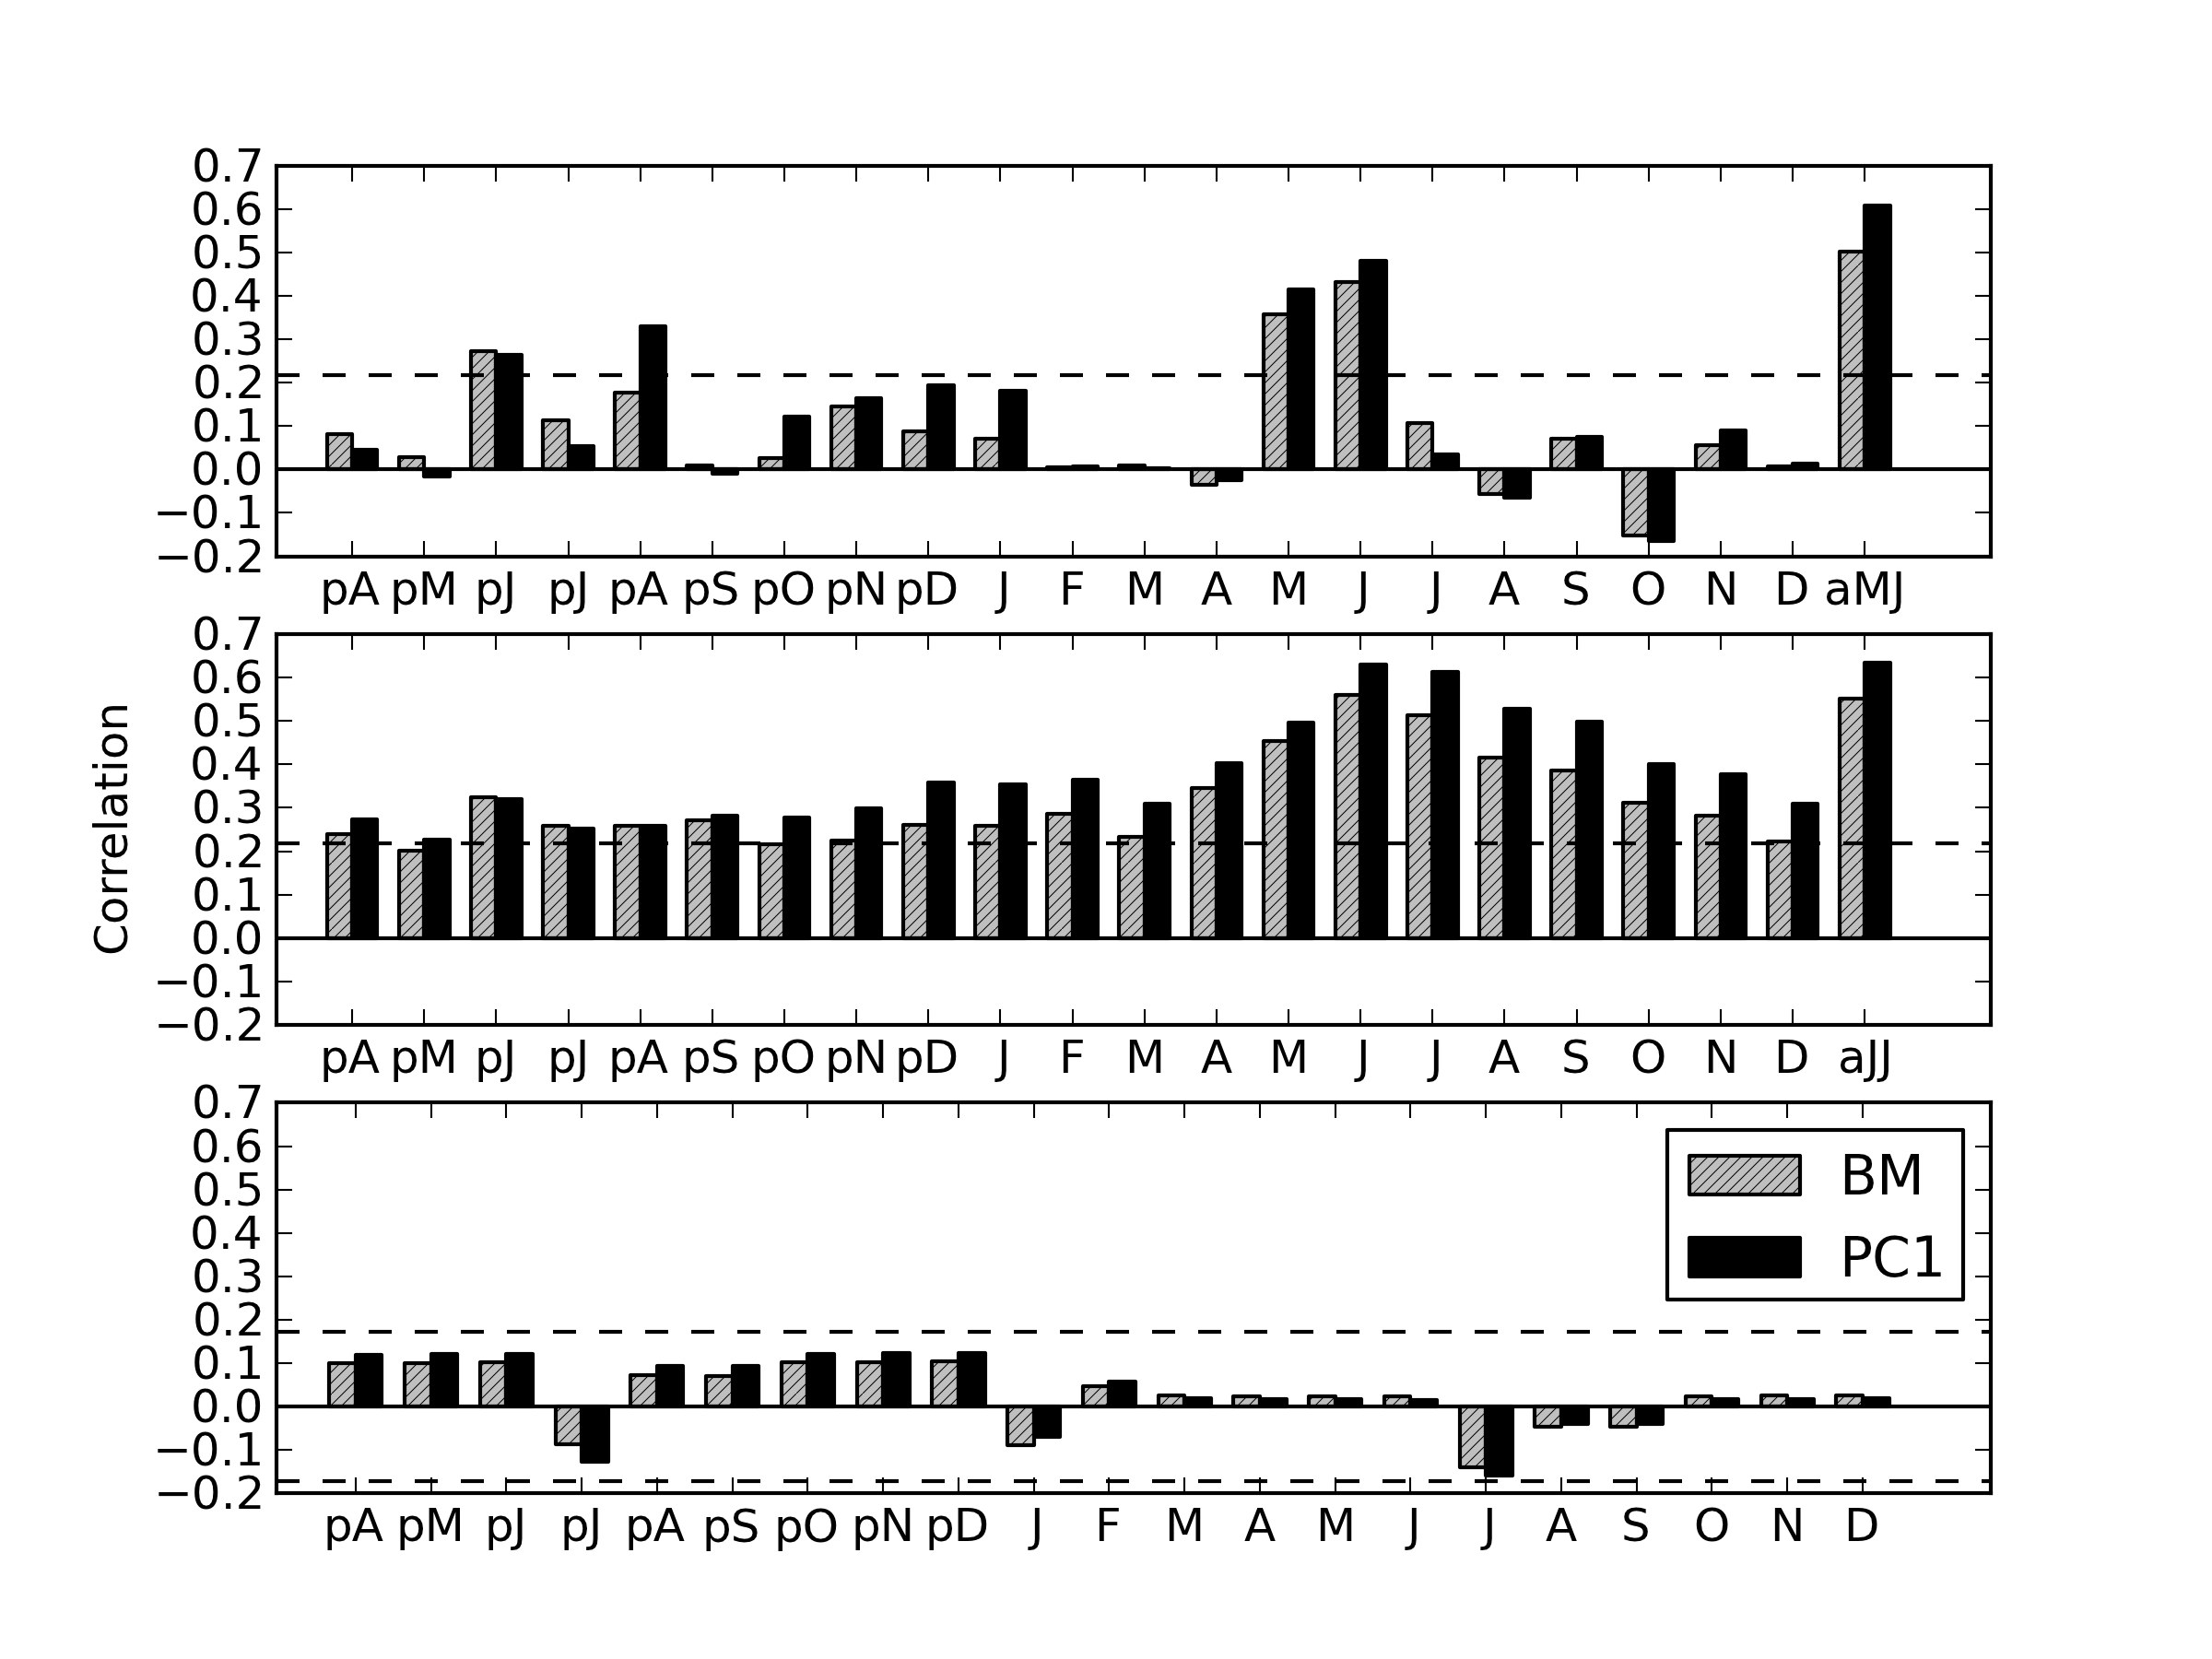
\includegraphics[width=5in]{figures/climCorr2.png}
\caption{Top: Correlation between the growth proxies (BM or PC1) and the monthly precipitation from previous April (pA) through December (D) as well as for average May and June (aMJ). Middle: Correlation between the growth proxies (BM or PC1) and average PDSI from previous April (pA) through December (D) as well as for average June and July (aJJ). Bottom: Correlation between the growth proxies (BM or PC1) and average monthly temperature from previous April (pA) through December (D).}
\label{fig:climCorr}
\end{figure}

%mjPR correlation map
\begin{figure}
\centering
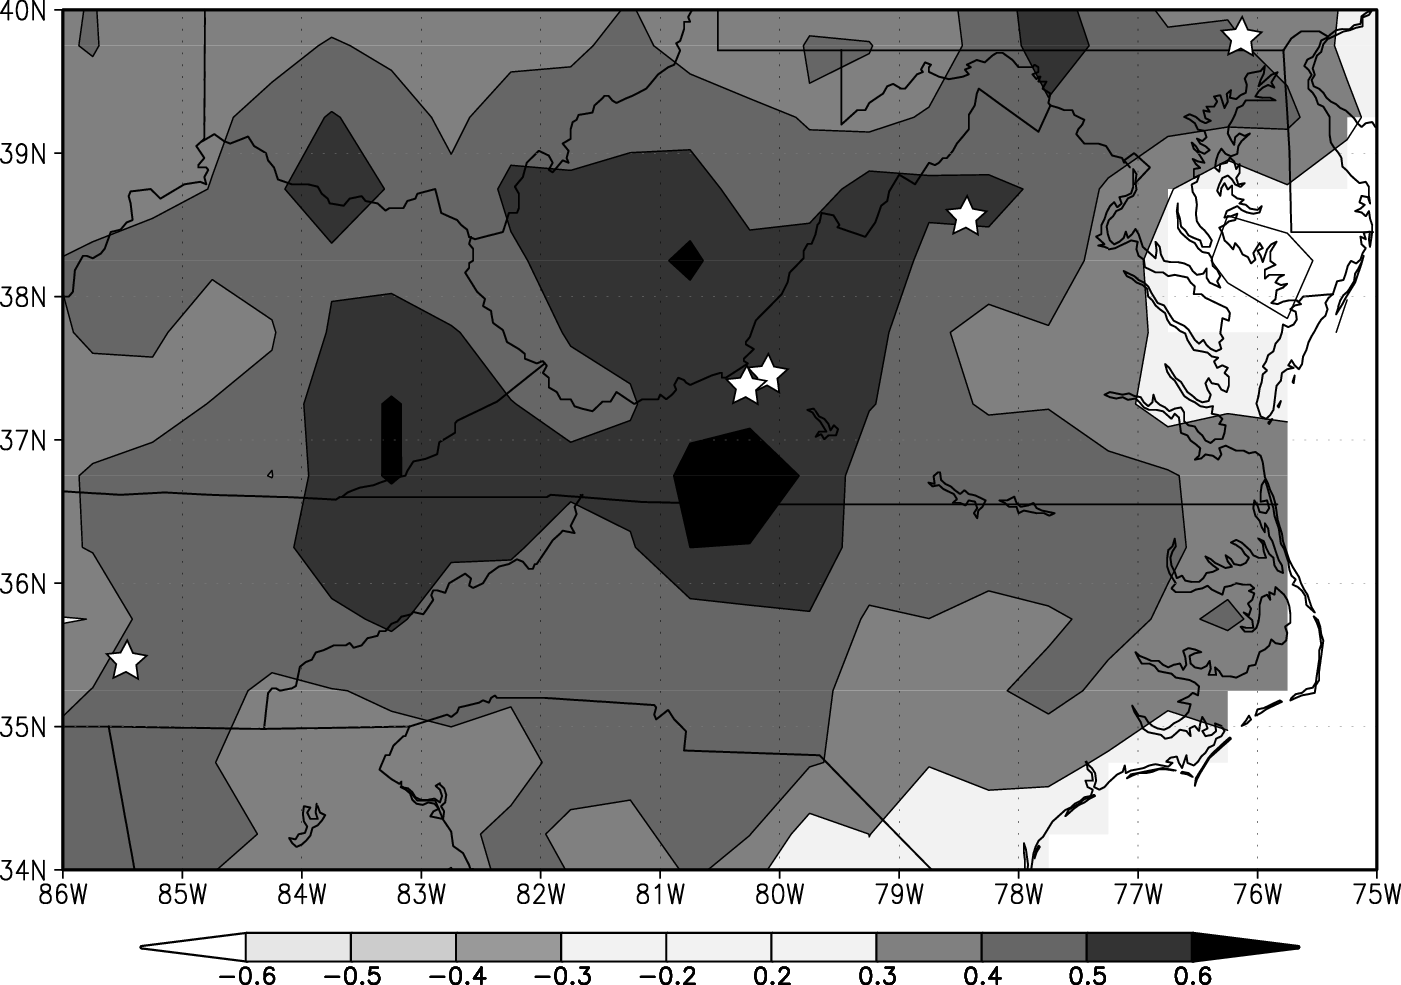
\includegraphics[width=5in]{figures/corrMapPrecipMJ_bw_annot.png}
\caption{Correlation map showing the correlation between the first principal component and averaged May-June precipitation. Stars indicate the locations of the sites where the tree-rings used to develop the contributing chronologies were sampled.}
\label{fig:precipCorrMap}
\end{figure}

%reconstruction
\begin{figure}
\centering
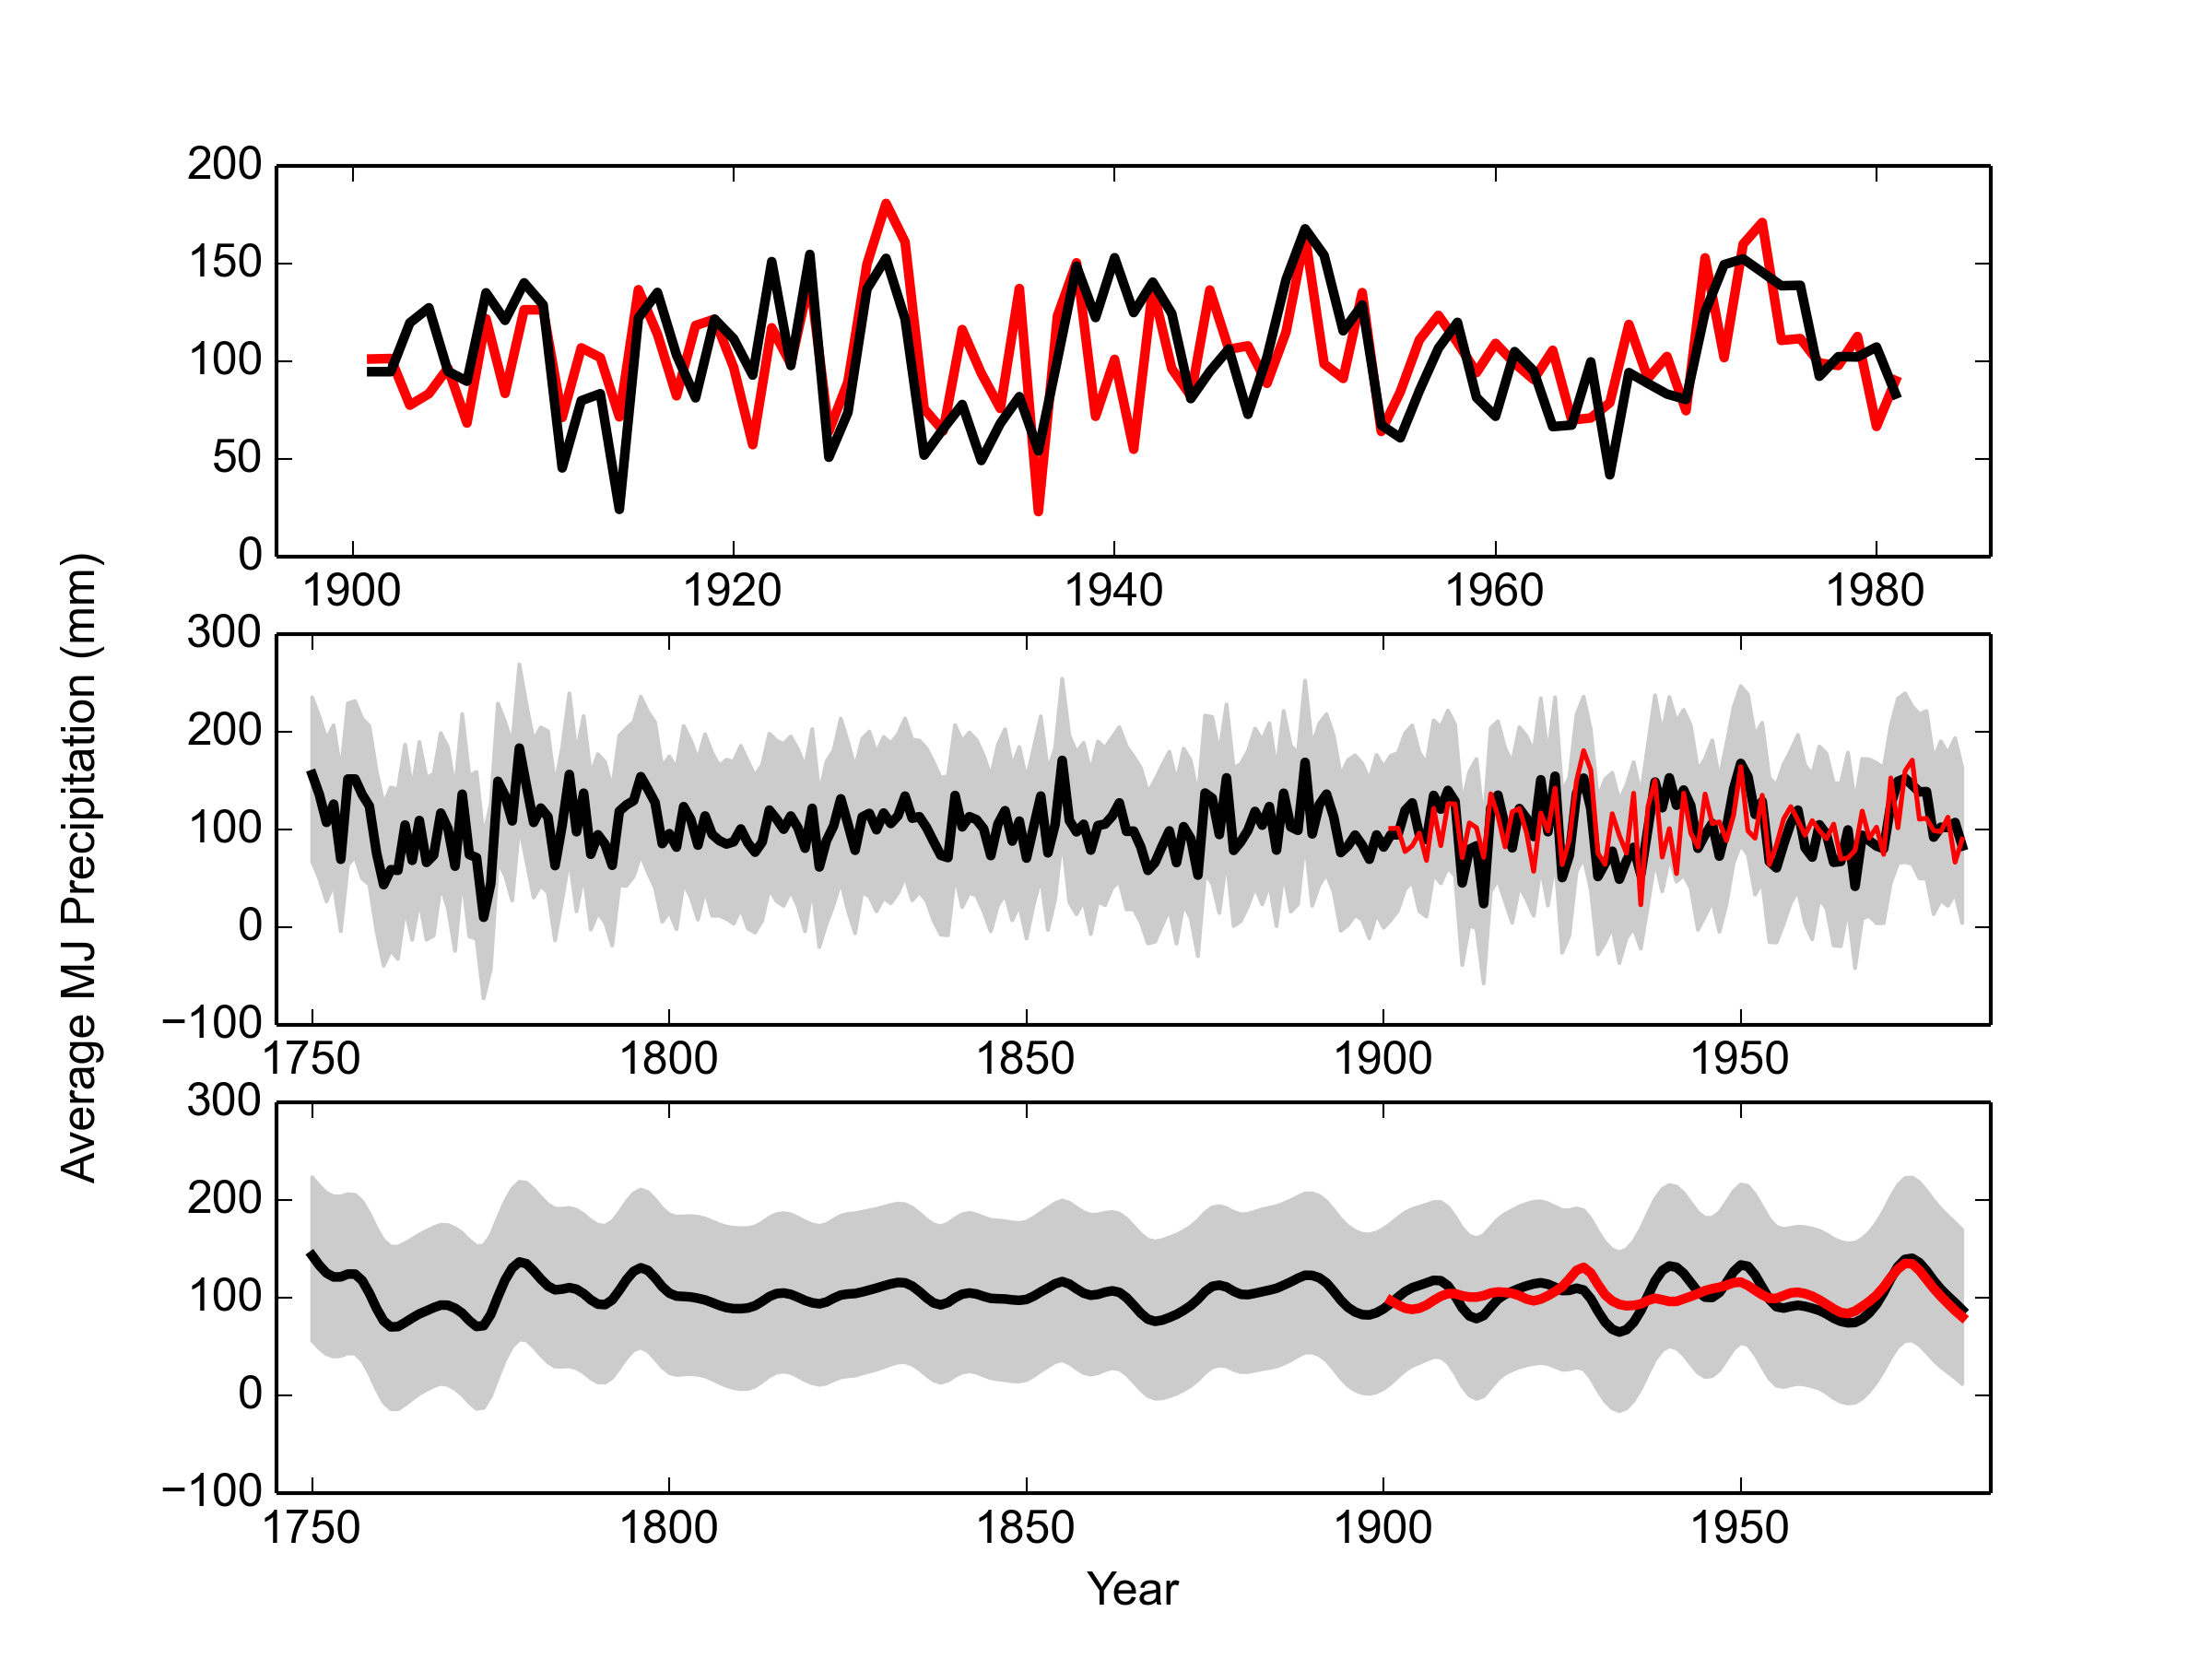
\includegraphics[width=5in]{figures/reconsmoothed.png}
\caption{Top panel: rSWV reconstruction (black curve) and the average May-June precipitation (red curve) for the 1901-1981 period of overlap. Middle panel: rSWV reconstruction (black curve) and the average May-June precipitation (red curve) for the 1750-1981 period of reconstruction. Bottom panel: Smoothed rSWV reconstruction (black curve) and 95\% credible interval (shaded grey area) back to 1750, and smoothed average May-June precipitation (red curve). Smoothing performed using a 10-year smoothing spline to highligh decadal-scale varibility.}
\label{fig:precipRecon}
\end{figure}

%spectral
\begin{figure}
\centering
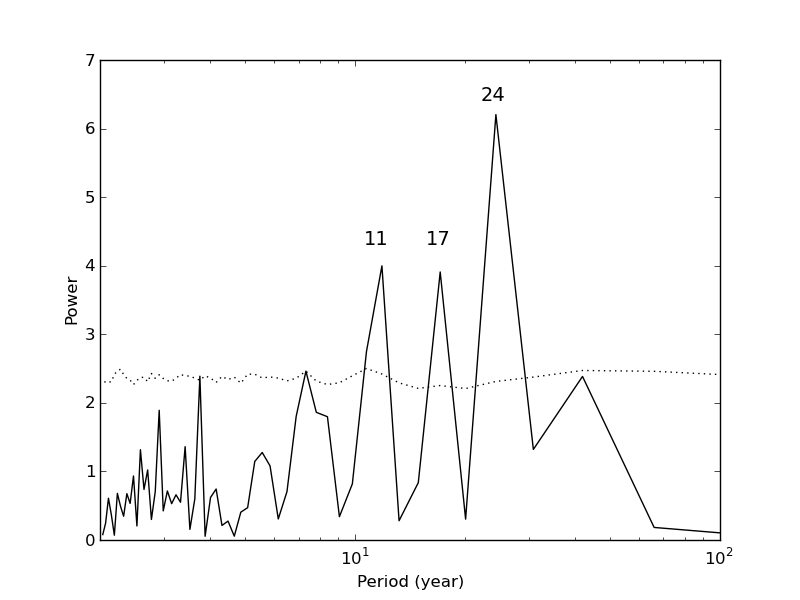
\includegraphics[width=5in]{figures/spectralRecon.png}
\caption{Periodogram of the SWV reconstruction showing spectral power peaks at approximately 11, 17, and 24 years.}
\label{fig:spectral}
\end{figure}

%%other recons
%\begin{figure}
%\centering
%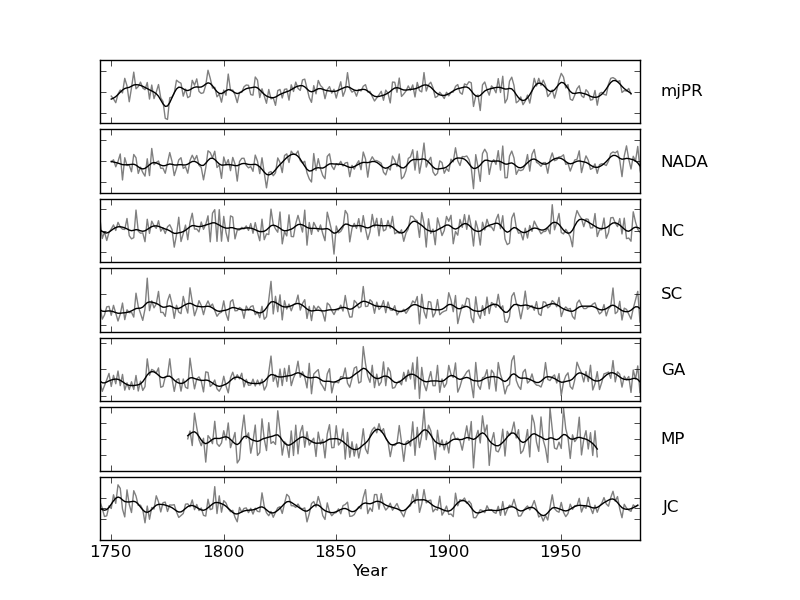
\includegraphics[width=5in]{figures/reconsStackedZoom.png}
%\caption{Time series plots showing annual- and decadal-scale variability for the mjPR and six compared moisture reconstructions for the period 1745-1985.}
%\label{fig:allReconsZoom}
%\end{figure}

%SWV recon and cook PDSI
\begin{figure}
\centering
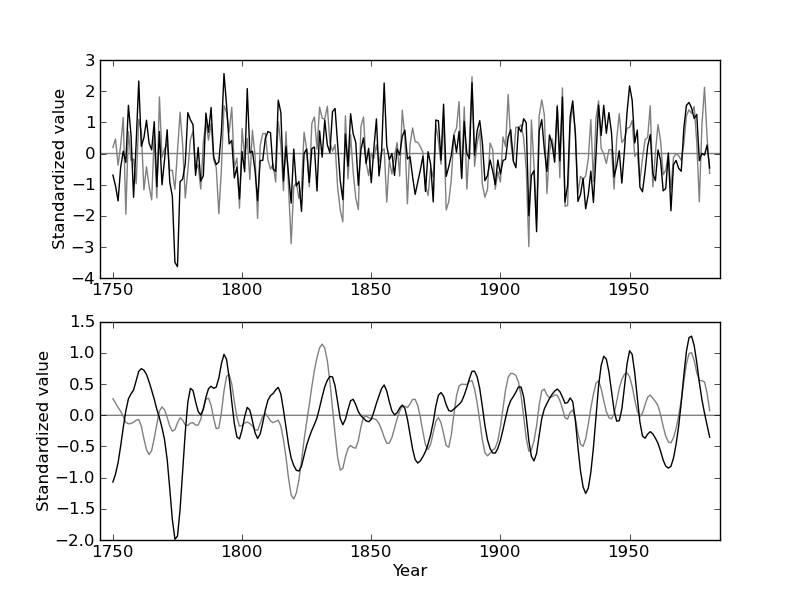
\includegraphics[width=5in]{figures/reconCompare.png}
\caption{The standardized rSWV average May-June precipitation reconstruction (black lines) and Cook PDSI (grey lines) reconstructions are plotted against time for comparison. The top panel shows the standardized reconstructions at an annual scale, while the bottom panel shows the time series after application of a 10-year smoothing spline to highlight the decadal-scale variability. Particularly notable differences include the year 1774, and the interval 1855-1863.}
\label{fig:reconCompare}
\end{figure}

%\begin{figure}
%\centering
%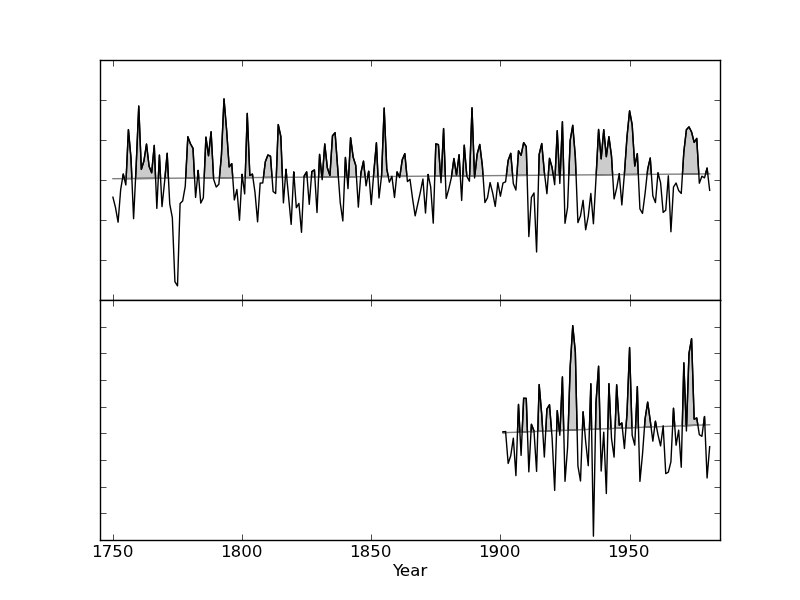
\includegraphics[width=5in]{figures/wetdry.png}
%\caption{The mjPR reconstruction (top panel) and the mjPR instrumental record (bottom panel). Lines show the best-fit regression line through the time series data to indicate any dominant trends. Areas falling above the best-fit lines and the time series data are shaded grey to indicate periods of higher precipitation. Note the correspondence of wetter and drier years between the top and bottom panels.}
%\label{fig:wetdry}
%\end{figure}

%\begin{figure}
%\centering
%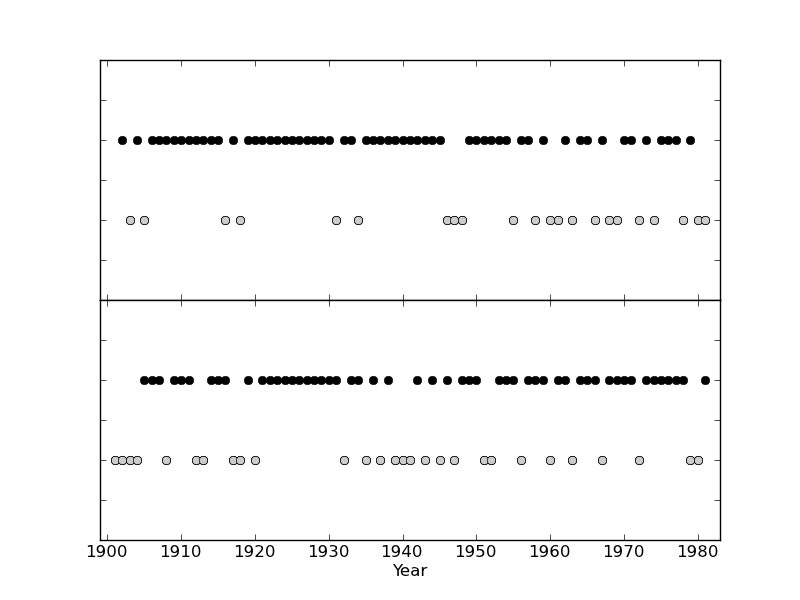
\includegraphics[width=5in]{figures/wetdry_dots.png}
%\caption{A representation of how the mjPR reconstruction and the mjPR instrumental record are changing with respect to each other. Top panels show a black dot if both time series were increasing or decreasing from the previous year to the year indicated, while the grey dots indicate that the time series changes are not synchronous. Time series show synchronous behavior with respect to this measure in 72\% of the years. Bottom panel shows a black dot if both time series are either above or below their respective best-fit trend lines, while the grey dots indicate asynchronous behavior. Time series show synchronous behavior with respect to this measure in 65\% of the years.}
%\label{fig:wetdry_dots}
%\end{figure}


%\begin{figure}
%\centering
%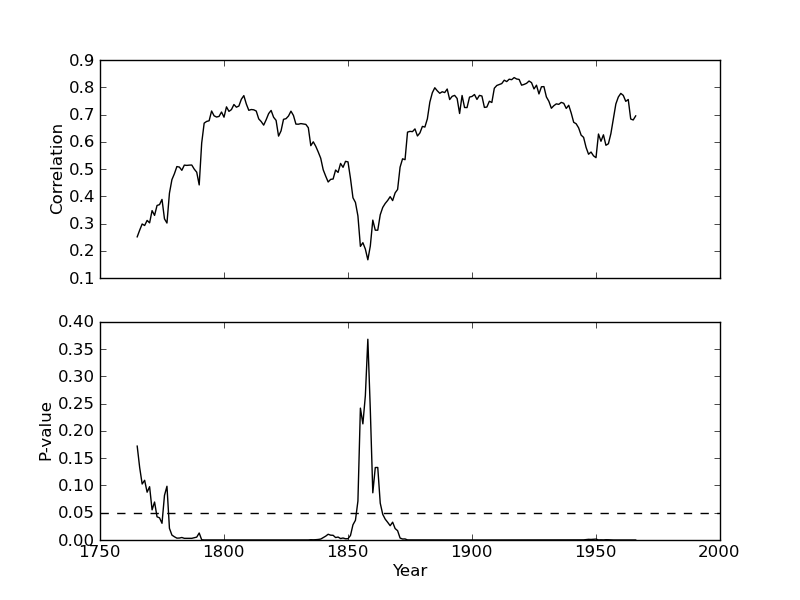
\includegraphics[width=5in]{figures/reconRunningCorr.png}
%\caption{A 31 year windowed correlation plot between the mjPR and Cook PDSI reconstructions shows the discrepancy during the 1855-1863 interval. In the top panel correlation values are plotted about window centers, while the bottom panel shows the corresponding p-value (black) as well as the line of significance (dashed).}
%\label{fig:reconRunningCorr}
%\end{figure}
%
%\begin{figure}
%\centering
%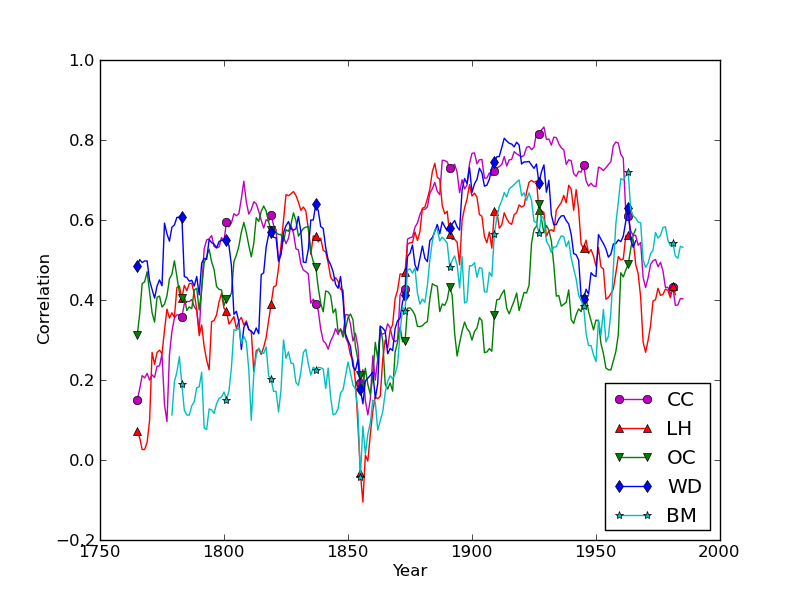
\includegraphics[width=5in]{figures/cookPdsiRunningCorr.png}
%\caption{A 31 year windowed correlation plot between each of the chronologies and the Cook PDSI reconstruction. Note the interval of abrupt poor correlation during the years 1855-1863.}
%\label{fig:cookRunningPdsiCorr}
%\end{figure}
%


%\begin{figure}
%\centering
%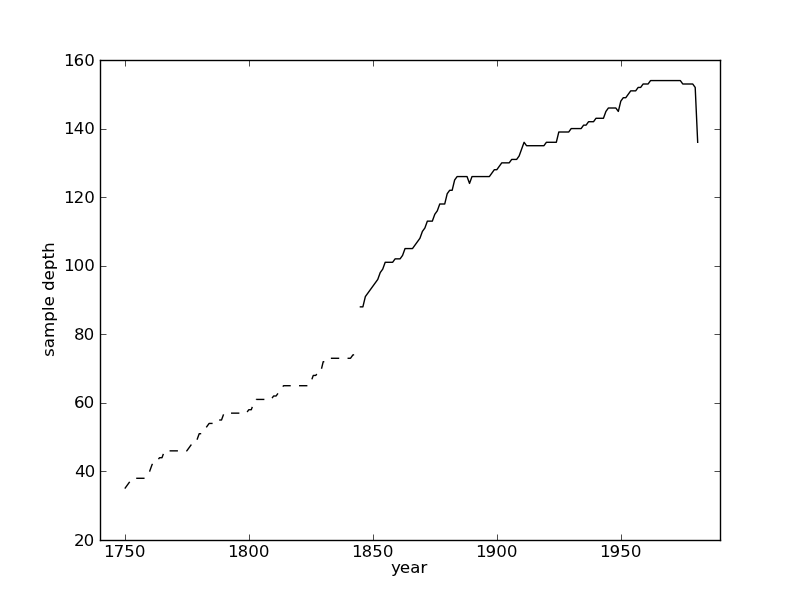
\includegraphics[width=5in]{figures/sample_depth.png}
%\caption{Sample depth by each year for the growth proxy obtained from the nested principal component analysis. The dashed line indicates the principal component which contained the years 1750-1844 with only four chronologies (WD, LH, CC, and OC), while the solid line indicates the principal component resulting from the analysis which used all five chronologies (BM, WD, LH, CC, and OC) and covered the years 1845-1981.}
%\label{fig:sampleDepth}
%\end{figure}

